% -*- root: article.tex -*-
Na Figura \ref{fig:all-violin}, apresentamos gráficos de violino da percepção dos desenvolvedores sobre os cheiros Android, tradicionais e códigos limpos. Além disso, relatamos a percepção dos desenvolvedores para cada uma das práticas em Android - Figura \ref{fig:smelly-violin}. No eixo y, 0 (zero) indica classes não percebidas pelos desenvolvedores como problemáticas (ou seja, responder "não" à pergunta: este código apresenta algum problema de design e/ou implementação?), enquanto valores de 1 a 5 indicam o nível de severidade para o problema percebido pelo desenvolvedor.

Os códigos limpos têm uma mediana de gravidade igual a 1,5. Isso indica que, como esperado, os desenvolvedores no geral, não consideram essas classes como problemáticas. Já os códigos afetados por cheiros Android têm mediana = 2 (Q3 = 4,25) e, portanto, são percebidos como problemáticas na maioria dos casos por desenvolvedores. Em relação aos cheiros tradicionais, a mediana de severidade é 3. Isso mostra que as classes afetadas por esses cheiros são percebidas pelos desenvolvedores como problemáticas. No entanto, embora essa diferença na percepção seja clara, observando-se os gráficos de violino na Figura 5.3a, tal diferença não é estatisticamente significativa (valor de p = 0,21). Conjeturamos que isso pode ser devido ao número limitado de pontos de dados (21 participantes).

\begin{figure}[!htb]
	\centering
	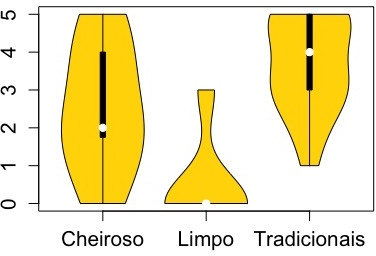
\includegraphics[width=0.3\textwidth]{plot-lcui-violin2.jpg}
	\caption{LCUI}
	\label{fig:CategoriaXRecorrencia}
\end{figure}

\begin{figure*}
\centering
\begin{subfigure}{.23\textwidth}
  \centering
  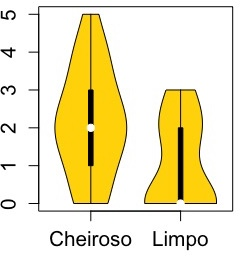
\includegraphics[width=.8\textwidth]{plot-recursos-violin2.jpg}
  \caption{Integrados}
  \label{fig:smelly-violin}
\end{subfigure}%
\begin{subfigure}{.23\textwidth}
  \centering
  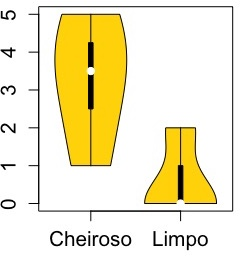
\includegraphics[width=.8\textwidth]{plot-lpa-violin.jpg}
  \caption{LPA}
  \label{fig:all-violin}
\end{subfigure}% 
\begin{subfigure}{.23\textwidth}
  \centering
  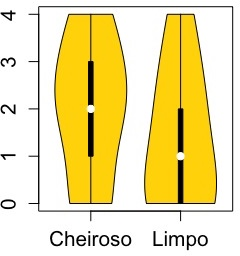
\includegraphics[width=.8\textwidth]{plot-rm-violin.jpg}
  \caption{RM}
  \label{fig:smelly-violin}
\end{subfigure}
\begin{subfigure}{.23\textwidth}
  \centering
  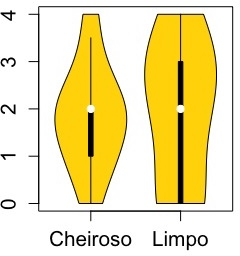
\includegraphics[width=.8\textwidth]{plot-nrd-violin.jpg}
  \caption{NRD}
  \label{fig:all-violin}
\end{subfigure}% 
\caption{Gráficos violinos individuais das más práticas que afetam recursos (LPA, RM e NRD).}
\label{fig:test}
\end{figure*}


% analise
% Próximo passo, salvar imagens violinos

ameacas a validade que é dificil selecionar código limpo